\chapter{Results}
%In this chapter we expect you to list and explain all the results that you have achieved. Pictures can be useful to explain the results. Think about this chapter as something similar to the demo of the oral presentation. You can also include pictures about use-cases (you can also decide to add use cases to the high level overview chapter).

The aim of the project has been successfully reached and the implemented PUF can check with a good accuracy that the device is the correct one.
Unfortunately, achieving 100\% accuracy in recognising the device is unfeasible. This is due to the fact that sometimes a few bits can change their standard value when the device is switched on.
For this reason, a non-null hamming distance can be present between the response received and the expected one.

Figure \ref{fig:Results} shows a graphical representation of the results obtained executing 1000 PUF authentications on the same device with 10 different challenge-response pairs.
It is possible to observe that by increasing the value of the thresholds for the hamming distance the number of responses recognised as correct increases.
Obviously, it would be incorrect to increase the value of the threshold too much because it would increase the risk of mistaking a device for another one, thus allowing attackers to counterfeit the original device. In this project, it was decided that a threshold equal to 4 is a good compromise between security and efficiency of the implementation.

\begin{figure}[tb]
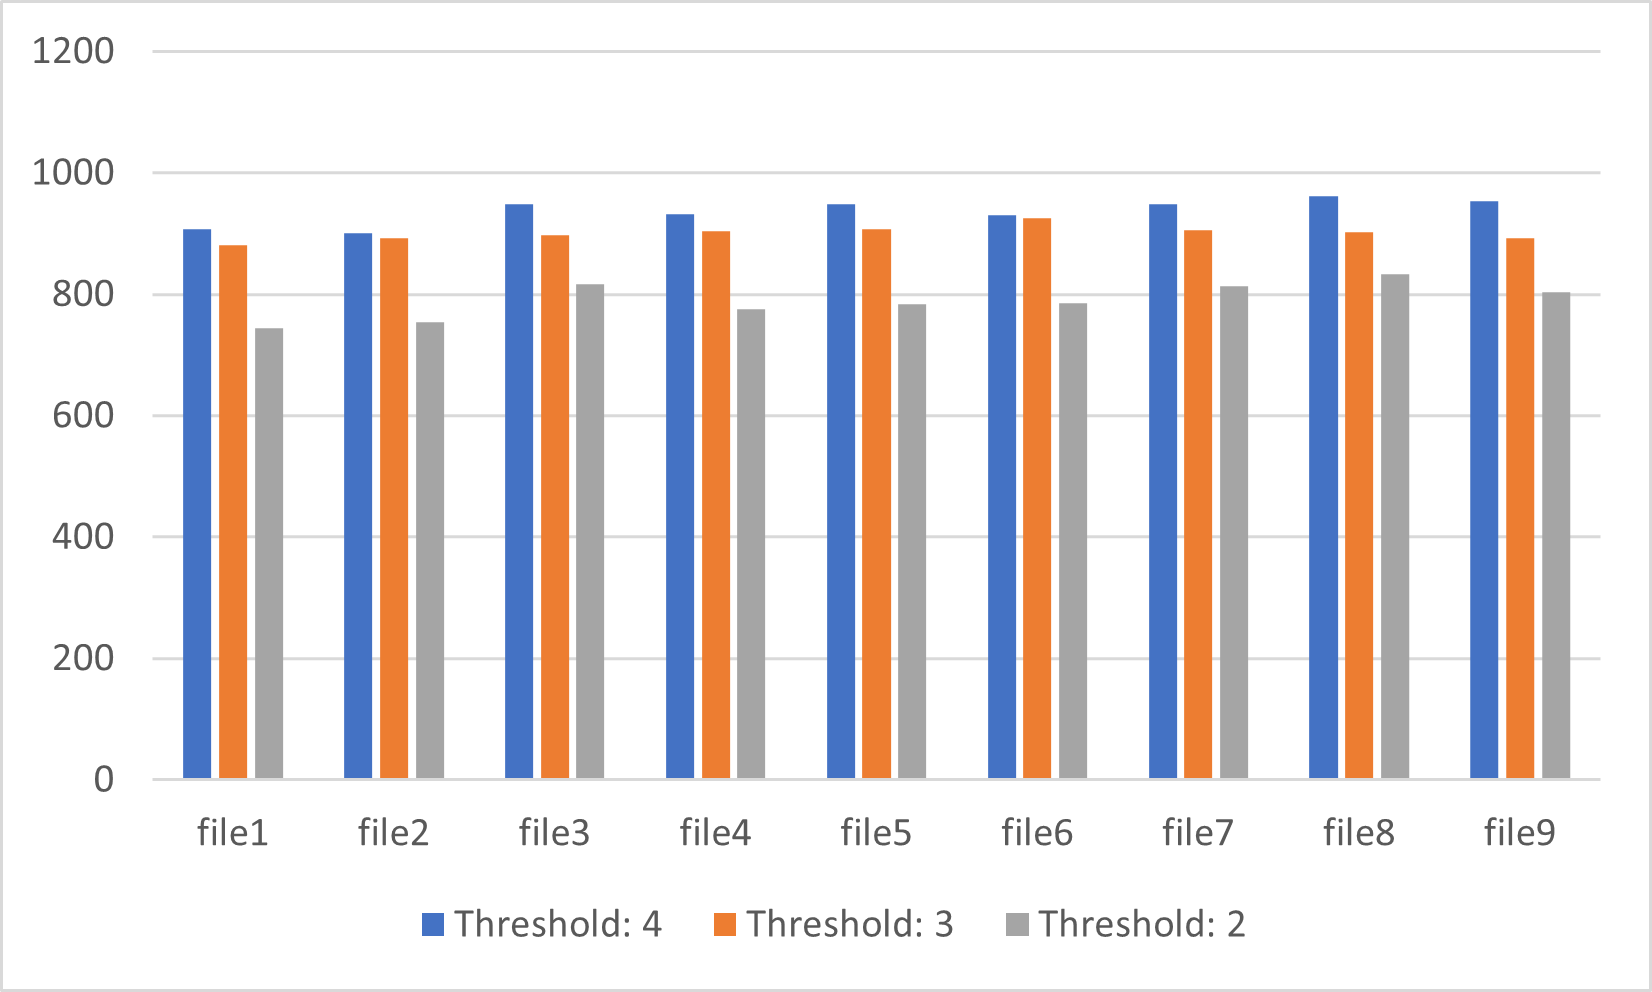
\includegraphics[width=\textwidth]{images/results.png}
\caption{Results of PUF authentications with different hamming distance thresholds. }
\label{fig:Results} % This is the image label, with which you can refer to the image in any document location
\end{figure}


\section{Known Issues}
%If there is any known issue, limitation, error, problem, etc...explain it in this section. Use a specific subsection for each known issue. Issues can be related to many things, including design issues.
One of the issues of this implementation is that it is not secure from the man-in-the-middle attack, since an attacker could easily steal the challenges and responses of the PUF.
There are some optimizations that can be done in order to avoid this kind of attack.
The main one would be to eliminate a challenge-response pair once it has been used: by doing this, even if an attacker manages to steal that pair, it will not be able to use it for a later authentication and replicant attacks can be therefore avoided.

Another type of security improvement is the encryption of the data in order to ensure confidentiality in the communication. The encryption should be used, in particular, during the first communication between device and host, i.e., when the device sends all the challenge-response pairs to the host.
It is also important to state that the type of encryption and the necessity to encrypt or not depend on the type of device and by the level of sensibility of the data that it can manage.

One more improvement could be to perform the responses match check on the board side. By doing this, the possibility of any manipulation of the response provided by the board before making the match check could be eliminated.


\section{Future Work}
Many are the implementations that can be done on this project, starting from the ones explained in the previous paragraph.
\\
\\
The main one could be to store the challenge-response in the file (host side) in the cipher way. In this way, if the file is stolen by an attacker he cannot be able to use the information.
\\
\\
Another one is to evaluate and store in a secure place the hash value of the file containing the challenge-response.
This kind of implementation can be used in order to ensure the integrity of the challenge-response of a particular device.
The idea consists in evaluating the hash value of the file before taking information from it and comparing it with the digest that we store in another place.
If the value is the same it means that the file is not corrupted.
%Adding a section about how to improve the project is not mandatory but it is useful to show that you actually understood the topics of the project and have ideas for improvements.



